\newif\ifvimbug
\vimbugfalse

\ifvimbug
\begin{document}
\fi

\exercise{Gaussian Processes}
\begin{questions}

%----------------------------------------------

\begin{question}{GP Regression}{10}
Implement a Gaussian Process to fit the target function $y = \sin(x) + \sin^2(x)$ with $x \in [0, 0.005, 0.01, 0.015, \ldots, 2\pi]$. Use a squared exponential kernel, an initial mean of 0 and assume a noise variance of 0.001. Begin with no target data points and, at each iteration, sample a new point from the target function according to the uncertainty of your GP (that is, sample the point where the uncertainty is the highest) and update it. Plot your GP (mean and two times standard deviation) after iterations 1, 2, 4, 8 and 16.
In each figure, plot also the true function as ground truth and add a new marker for each new sampled point. Attach a snippet of your code.

\begin{answer}
The following pictures demonstrate our results with implementing the Gaussian Process and trying to fit the given target function. We shall notice that Gaussian Processes are a non-parametric model, meaning that they have an infinite number of parameters or that the data is our parameter. This means, that a Gaussian Process will always have a maximum uncercainity at the point where we have the least amount of data. Since the numpy linspace function spaces data points evenly out, we just need to increase the amount of points that we want to generate points which are at the maximum uncertainity of the Gaussian Process, no futher calculations required. 

I want also point out that it seems not be a good idea to naively invert the Kernel-Matrix in order to calculate the mean. Instead we need to solve two different sets of linear equation systems. In this deparment our code borrows from Nando de Freitas (Professor at UBC) who has a fantastic lecture on Youtube, talking about the numerical problems in Gaussian Processes.
\end{answer}

Lets take a look at this beautfiul graph \ref{fig:GP_all} showing all 16 iterations of the Gaussian Process. We can see that our how the standard derivation continously shrinkes when increasing the number of training points. 
\begin{figure}[H]
	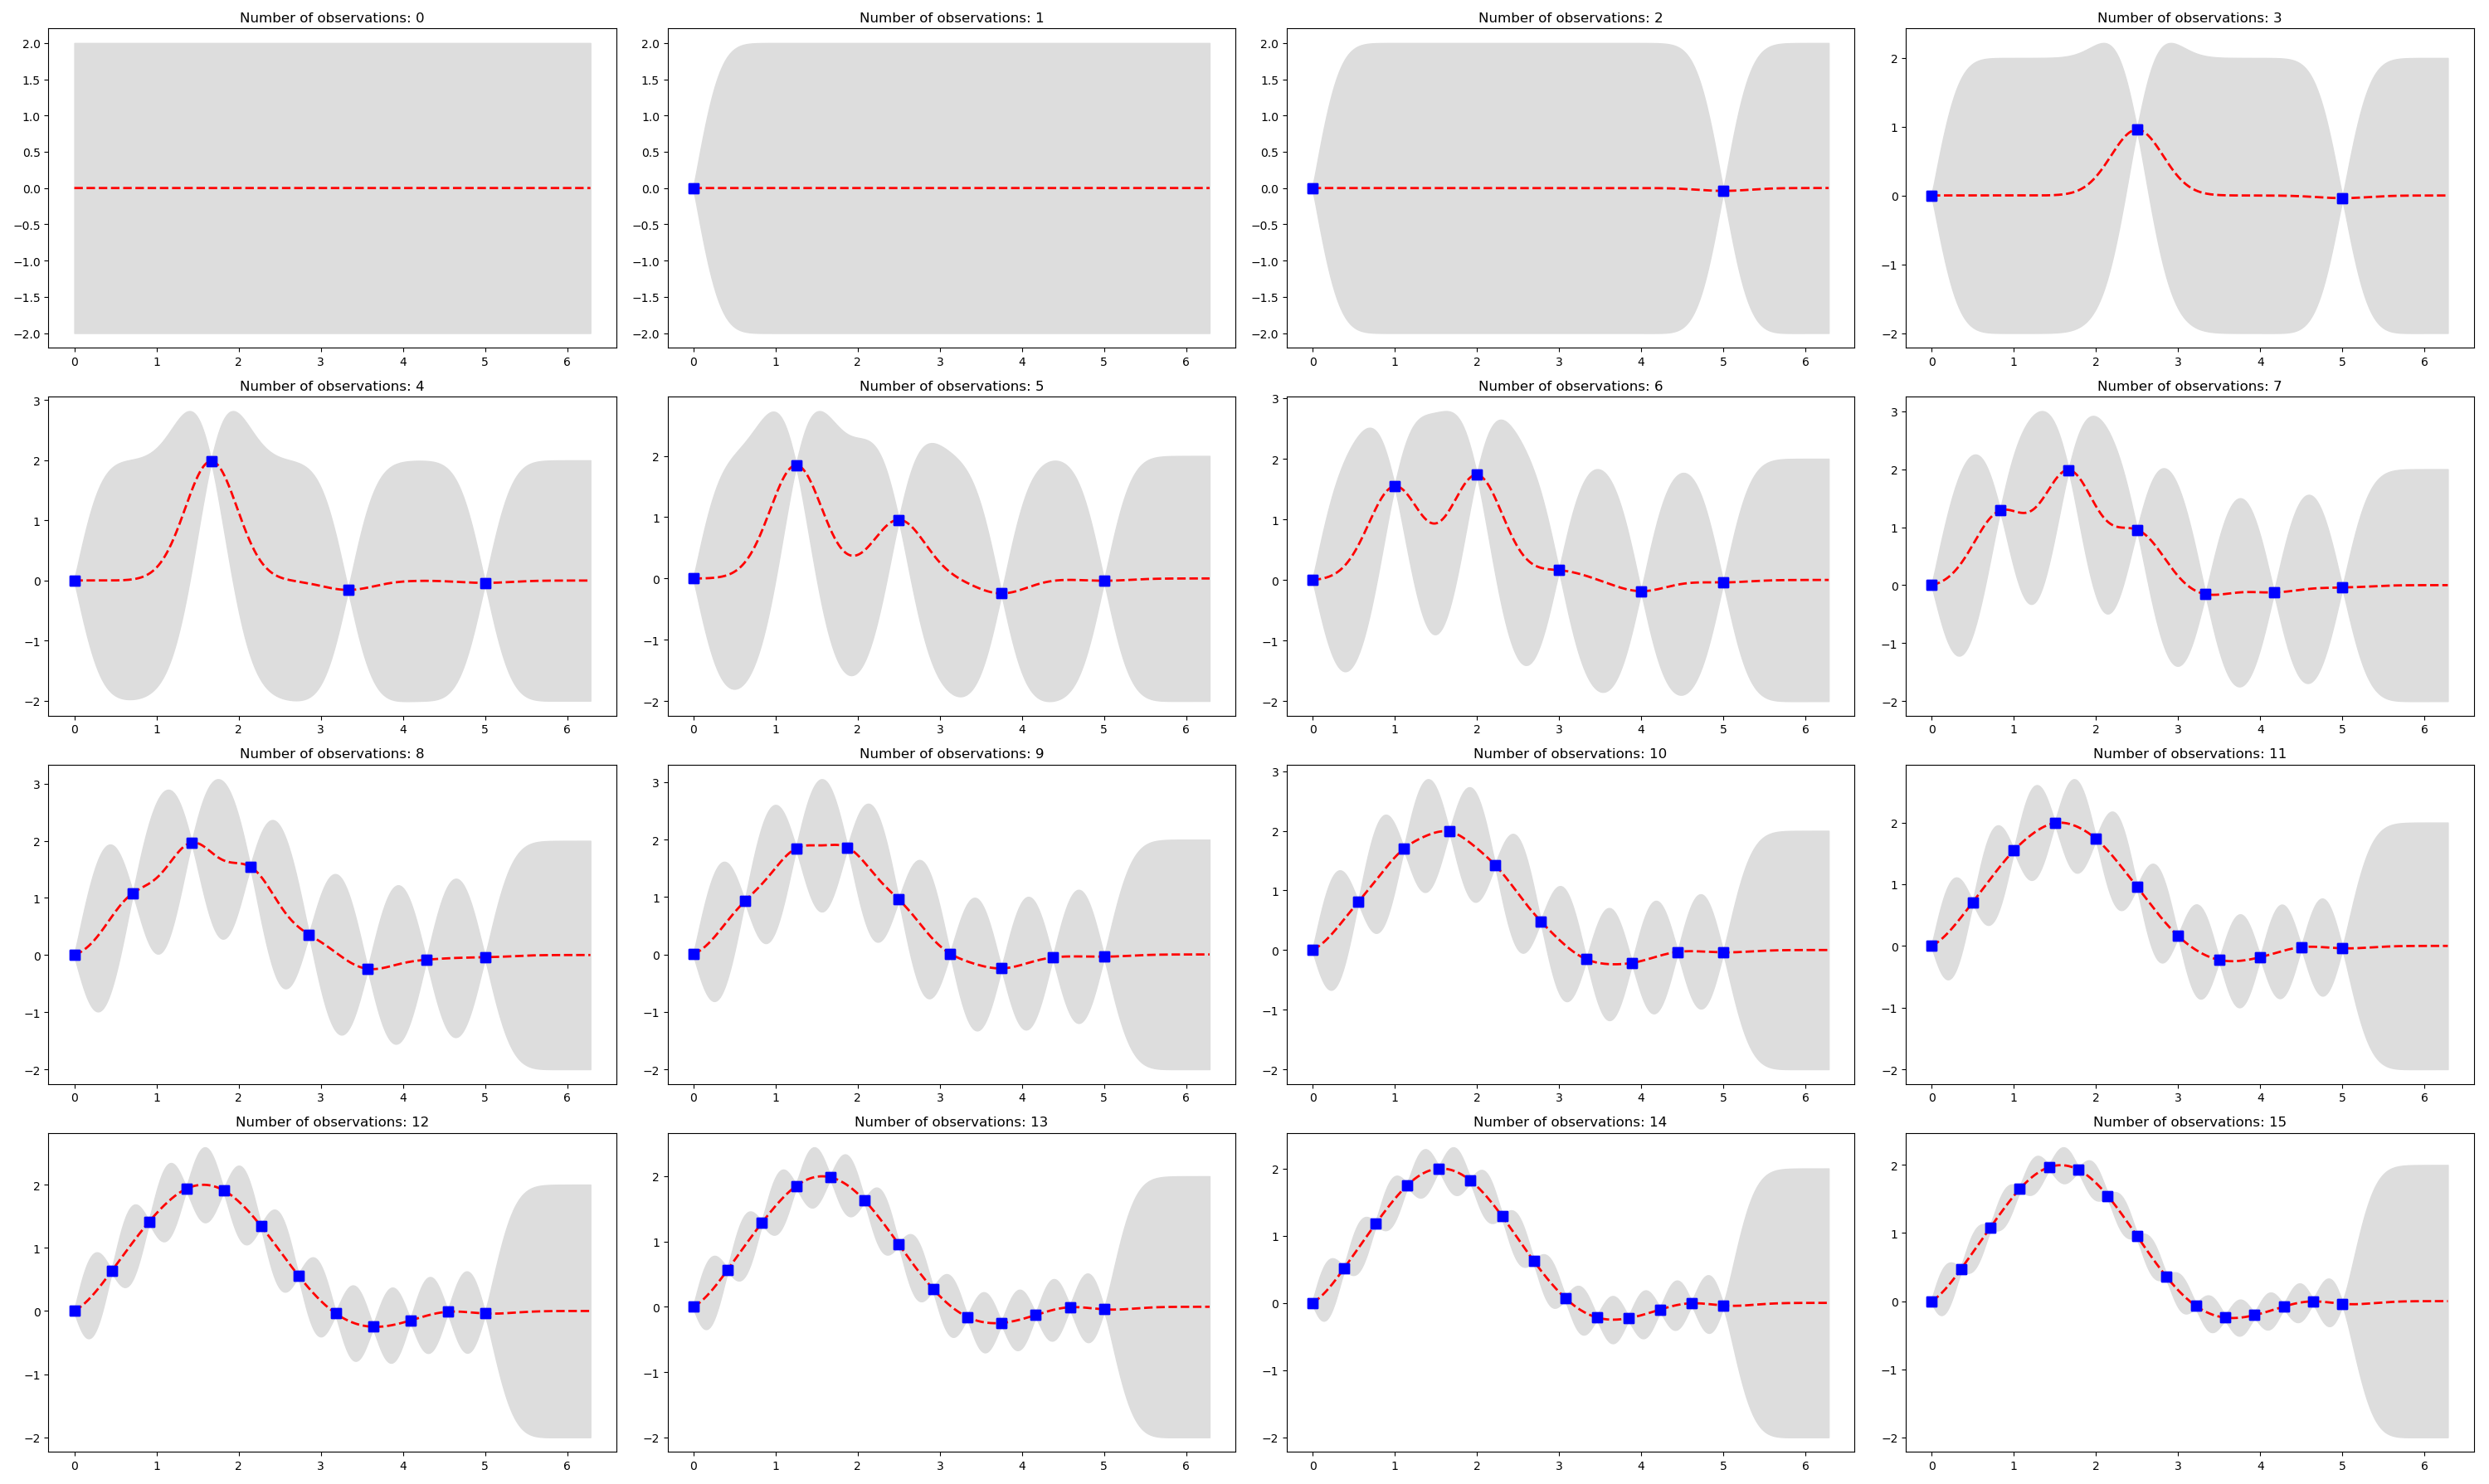
\includegraphics[width=1.0\linewidth]{pictures/GP_all_plots.png}
	\centering
	\caption{An overview of all 16 iterations for the Gaussian Process. It's beautfiul isn't it?}
	\label{fig:GP_all}
\end{figure}

In case you're overwelmed by the information density of this graph, here are the extracted versions for first \ref{fig:GP_1}, second \ref{fig:GP_2}, fourth \ref{fig:GP_4}, eight \ref{fig:GP_8} and sixtheen iteration \ref{fig:GP_16} respectivly, showing n-1 number of observations, since we start with zero observations.
\begin{figure}[H]
	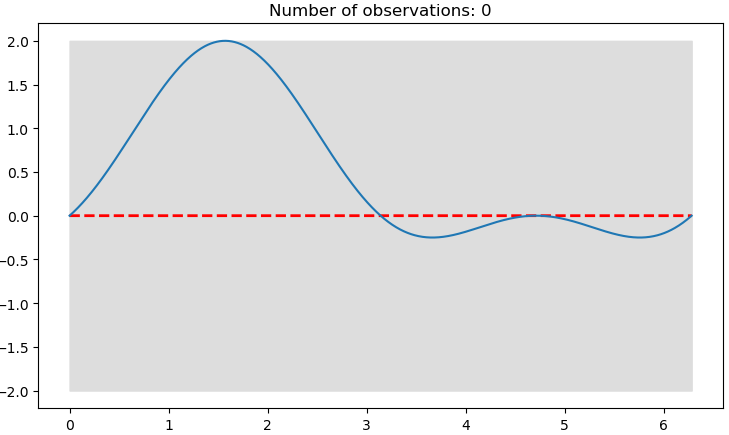
\includegraphics[width=0.6\linewidth]{pictures/GP_plot_1.png}
	\centering
	\caption{Gaussian Process for the first iteration with zero observations. We assume zero mean.}
	\label{fig:GP_1}
\end{figure}

\begin{figure}[H]
	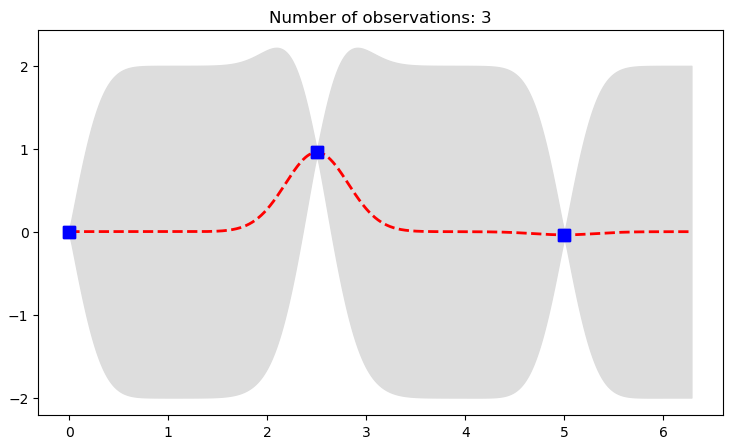
\includegraphics[width=0.6\linewidth]{pictures/GP_plot_2.png}
	\centering
	\caption{Gaussian Process for the second iteration with one observations.}
	\label{fig:GP_2}
\end{figure}

\begin{figure}[H]
	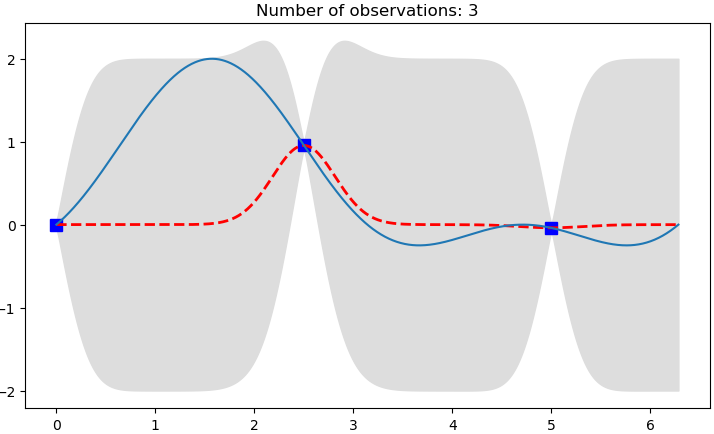
\includegraphics[width=0.6\linewidth]{pictures/GP_plot_4.png}
	\centering
	\caption{Gaussian Process for the fourth iteration with three observations.}
	\label{fig:GP_4}
\end{figure}

\begin{figure}[H]
	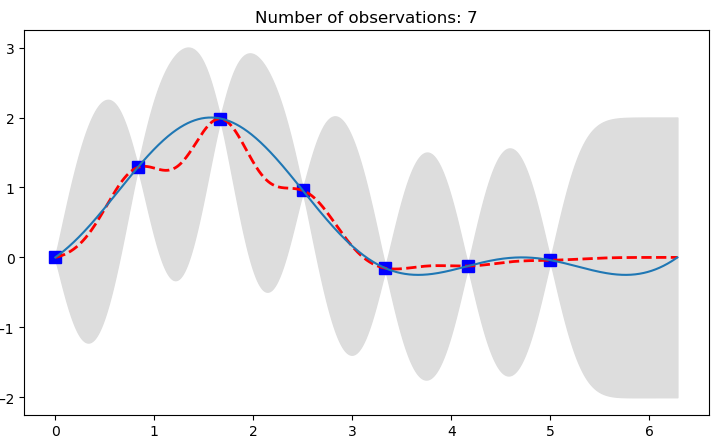
\includegraphics[width=0.6\linewidth]{pictures/GP_plot_8.png}
	\centering
	\caption{Gaussian Process for the eight iteration with seven observations.}
	\label{fig:GP_8}
\end{figure}

\begin{figure}[H]
	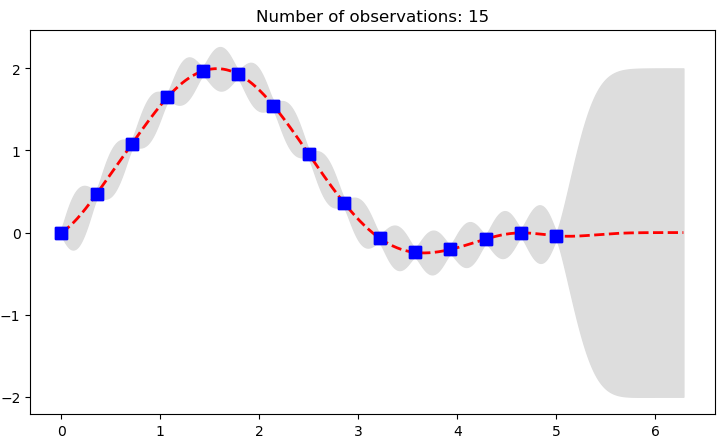
\includegraphics[width=0.6\linewidth]{pictures/GP_plot_16.png}
	\centering
	\caption{Gaussian Process for the sixteenth iteration with fifteen observations.}
	\label{fig:GP_16}
\end{figure}

\lstinputlisting[language=Python]{code/gp.py}
\end{question}

%----------------------------------------------

\end{questions}
